\documentclass[
  10pt,
  b5paper,
  %a4paper,
  %draft,
  oneside
]{thesis}

% meta
\hypersetup{
  pdftitle={User Meta Modeling},
  pdfauthor={Olav Bjørkøy},
  pdfcreator={Olav Bjørkøy},
  pdfsubject={Aggregating User Modeling Methods, on a personal level},
  pdfkeywords={user modeling} {ai} {meta modeling}
}

\begin{document}
  
  %\frontmatter
  %  \thispagestyle{empty} 

\begin{narrow}

\null\vspace{6em}

{
  \centering
  \LARGE{Stacked Recommenders}\\
  \vspace{1em}
  
  \itshape
  \color{red}
  \large{Adaptive User Model Aggregation}\\
  \large{Through Individual Accuracy Estimation}\\
}

\vspace{5em}

{
  \centering
  \itshape
  Assignment\\
}
\vspace{1em}

Study how to aggregate user models on a per-user and per-item
basis when combining results from complementing modeling algorithms.

Create a flexible algorithm that combines multiple predictions
into one coherent result.
Utilize the resulting aggregation algorithm
to provide personalized search in an information retrieval system.

\end{narrow}
\vfill
\clearpage


\clearpage

\tableofcontents*
\thispagestyle{empty}
\clearpage

\listoffigures*
\thispagestyle{empty}
\clearpage



    
  \mainmatter
    
    %\chapter{Introduction}
    %  \label{chap:intro}

Information is a curious thing:
having too much can be as harmful as having no information at all.
While lacking information is an obvious problem,
too much leads to information overload,
where relevant content drowns in irrelevant noise.
As the amount of information grows,
our ability to make informed descisions quickly diminish.
Our amount of available attention is limited, and each new bit
of information consumes it further
\cite[p1]{Davenport2001}.

However, while people struggle with excessive information,
algorithms in artificial intelligence simply can not get enough.
\citet[p1]{Halevy2009} calls this the \emph{unreasonable effectiveness of data}:
perhaps surprisingly, more data often trumps more efficient algorithms.
\citet[p3]{Banko2001} shows how traditional algorithms can be substantially
improved by giving them a lot more data to work with.
As much as researchers chase elegant algorithms,
finding more data to work with may be time better spent.

Few places is this difference of users and computers more apparent than in \emph{recommender systems}.
A recommender system is a technique in user modeling to estimate the relevance of an item to a user.
An item can be anything: documents, websites, movies, events, or indeed, other users.
These techniques are especially prolific on the Web: 
wherever there is personalized recommendations of news, books, movies,
articles, social connections, search results, et cetera, recommender systems are the tools
working behind the scenes.

Modern recommender systems often embrace the unreasonable effectiveness of data,
by combining multiple recommender methods that predict relevance in various ways.
By considering different aspects of users and items when making predictions,
the methods provide quite complex predictions that rely on much evidence.
These systems can use data such as search query logs, relevance judgements from similar users,
social connections and much more, as we shall soon see.
For example, \citet[p1]{Bell2007} took this to its logical conclusion by 
combining an astonishing 107 different recommenders when winning the Netflix recommendation competition
(see \citet{Linden2009}).

While the name might seem constraining, recommender systems are incredibly powerful tools.
If we can accurately predict how each user will react to each item, the information overload problem would be solved.
Likewise, chronological sorting of items would be a figment of a simplistic past.
User interfaces could provide optimal selection and placement of information to each user.

However, despite their apparent power, in the real world, recommender systems are often confined
to menial tasks like creating small lists of recommended items, 
or meekly suggesting similar items to the ones being considered by a user.
The primary examples are recommended movies, social connections or news articles.
Seldom are their potential reached by creating completely adaptive
content systems, that work hard to mitigate any signs of information overload.

We posit that traditional recommender systems have an important weakness.
There exists an underlying, misplaced subjectivity to relevance prediction.
This fundamental weakness hinders the full adoption of these systems.

Consider this: 
when a method is developed or selected for use in a recommender system,
a concious descision of which approach to use is made.
Before any user modeling is performed, the researcher or developer selects
one or more methods that is thought to best model every user and item in the system.
While the methods themselves may perform well, their selection
reflects how whoever created the system assumes how each user
can and \emph{should} be modeled. This underlying subjectivity is not desirable.
We call this the \emph{latent subjectivity problem}.

Examples are not hard to come by.
For instance, while one user might appreciate social
influence in their search results, another user might not.
While one user might find frequency of communication maps well to relevance,
another might not. 
One user might feel the similarity of movie titles are a good predictor,
while another might be more influenced by production year.
The exact differences are not important --- what is important is that they exist.

The same goes for items: while one item might best be judged by its content,
another might be better described by previous ratings from other users.
One item's relevance may be closely tied to when it was created,
while other items may be timeless.

Should it not be up to each user to implicitly decide which method best describes their preferences?
And, considering the vast scope of items we can come by, will the selected
methods perform similarly for every item?
How much each algorithm is used should be used implicitly and automatically
based on how well they have previously worked for the current user.
At the same time, each algorithm should only be seriously considered
when considering items is has worked well for in the past.
Without this adaptability, it may be hard for recommender systems
to gain traction in scenarios with widely differing users and items.

Another way of explaining the latent subjectivity problem is that 
\emph{user modeling methods are dependent on the subjective assumptions of their creators}.
In other words, a modeling method use some aspect of available data to make predictions,
and this aspect is chosen by whoever creates the system.

Aggregate modeling methods face the same problem of misplaced subjectivity: 
Aggregation is done on a generalized, global level,
where each user and item is expected to place the same importance on each modeling method.
While the aggregation is of course selected to minimize some error over a testing set,
the subjective nature remains: the compiled aggregation is a generalization,
treating all users the same --- hardly a goal of user modeling.

We propose a novel method called \emph{stacked recommenders}, where these descisions are left to each user and item,
providing an extra level of abstraction and personalization.
The descisions are implict, and happens in the background, without any extra interaction required.
This leaves the subjective nature of selecting ways to model users and items where it should be:
in the hands of each individual user, and dependent on each specific item, without any extraneous effort.
If each method of relevance prediction is \emph{only used} based on how well it performs for each element,
any possibly applicable recommender system suddenly becomes a worthy addition to the system.

As far as we know, this kind of adaptive prediction aggregation has not been done before.
If we can construct an ensemble system that leverage each algorithm
based on how well it will perform for the current user and item,
we will have come closer to solving the latent subjectivity problem.

Can stacked recommenders help standard recommender systems reach their full potential?
Can a system where each user and item implicitly decides how they should be modeled outperform traditional approaches?
\emph{That is the main research question of this paper}.

%\hr

This paper is structured as follows.
Chapter \ref{chap:theory} will present the background theory needed to develop our modeling method:
the information overload problem, user modeling and recommender systems and personalized search. 
Chapter \ref{chap:methods} will build the \emph{stacked recommenders} approach from the ground up.
Our approach will allow us to adaptively combine different recommenders
on a per-user and per-item level, sidestepping the the latent subjectivity problem.
Chapter \ref{chap:results} will test three hypotheses and experiment with our newly built model.
We will try prediction aggregating for singular items, and rank aggregation for personalized search.
Finally, Chapter \ref{chap:discussion} will discuss the implications of our results,
their limitations, our contributions and suggest future work.




    \chapter{Theory}
      %This chapter introduces the basic theories of 
user modeling, recommender systems, personalized search and user model aggregation.

\section{User Modeling}

User Modeling (UM) is all about adapting an application to its users.
This has the potential to solve three problems that many applications face:

\begin{enumerate}

\item \emph{Information overload} conveys the act of receiving \emph{too much information} \cite[p13]{Bjorkoy2010d}. 
The problem is apparent in situations where decisional accuracy turns from improving with more information, to being hindered by too much irrelevant data \cite{Eppler2004}. 
The overload is often likened to a \emph{paradox of choice}, as there may be no problem acquiring the relevant information, but rather identifying this information once acquired. As put by \cite{Edmunds2000}: "The paradox --- a surfeit of information and a paucity of useful information."
While normal cases of such overload typically result in feelings of being overwhelmed and out of control, \cite{Bawden2008} points to studies linking extreme cases to various psychological conditions related to stressful situations, lost attention span, increased distractibility and general impatience.
\footnote{Information overload is a widespread phenomenon, with as many definitions as there are fields experiencing the problem. Examples include \emph{sensory overload}, \emph{cognitive overload} and \emph{information anxiety} \citep{Eppler2004}.}

\item \emph{Content discovery} is closely related to information overload. When the amount of information grows, 
discovering and evaluating new content becomes more difficult. 

\item \emph{Presentational preferences} differ between users. From simple preferences to actual physical contraints. 

\end{enumerate}

\cite{Kirsh2000} argues that "the psychological effort of making hard decisions about \emph{pushed} information is the first cause of cognitive overload." According to \citeauthor{Kirsh2000}, there will never be a fully satisfiable solution to the problem of overabundant information, but that optimal environments can be designed to increase productivity and reduce the level of stress through careful consideration of the user's needs. 

The fields of Artificial Intelligence (AI) and Human-Computer Interaction (HCI) share a common goal solving these problems through user modeling. 
However, as described by \cite{Lieberman2009}, their efforts are seldom combined: while ai researchers often view contributions from hci as trivial cosmetics, the hci camp
tends to view ai as unreliable and unpredictable --- surefire aspects of poor interaction design.

In AI, user modeling refers to precise algorithms and methods that infer knowledge about a user based on past interaction 
(\cite{Pazzani2007, Smyth2007, Alshamri2008, Resnick1994})  
By examining previous actions, predictions can be made of how the user will react to future information. This new knowledge is then embedded in a model of the user, which can predict future actions and reactions. 
For instance, an individual user model may predict how interesting an unseen article will be to a user, based on previous feedback on similar articles or the feedback of similar users.

HCI aims to meet user demands for interaction. 
User modeling plays a crucial role in this task. 
Unlike the formal user modeling methods of AI, user models in HCI are often cognitive approximations, manually developed by researchers to describe different types of users 
(\cite{Fischer2001, Jameson2009, Cato2001})
These models are then utilized by interaction designers to properly design the computer interface based on a models predictions of its user’s preferences.
\cite{Totterdell1990} describes user modeling in interaction design as a collection of deferred parameters: "The designer defers some of the design parameters such that they can be selected or fixed by features of the environment at the time of interaction [...] Conventional systems are special cases of adaptive systems in which the parameters have been pre-set."

In earlier years, the field of user modeling was fragmented by its multidiscipline nature. 
However, as described by \cite{Kobsa2001}, recent research has blurred the lines between the AI and HCI in user modeling.

\begin{eqnarray}
  \mathrm{UM} = (Items, Users, Models, Prediction)
\end{eqnarray}









the modeling problem: model+prediction

the core problem: estimating preferences

getting past 80\%

the efficiency of data


\subsection{Recommender Systems}

\begin{eqnarray}
  \mathrm{RS} = (Items, Users, Ratings, Framework, Method)
\end{eqnarray}

Users, items and ratings

machine learning fundamentals

modeling or heuristics

Taxonomy: model/heur, granularity, temporality, agents

\subsection{Approaches}

Modeling approaches

Heuristic approaches


\section{Personalized Search}

Information retrieval (+ information overload)

An Information Retrielal Model is a quadruple \citep[p23]{Baeza-Yates1999}:

\begin{eqnarray}
  \mathrm{IR} = (Documents, Queries, Framework, ranking(q_i, d_i))
\end{eqnarray}

Common metrics

Personalized metrics

Relation to user modeling


\section{Aggregate Modeling}

\begin{eqnarray}
  \mathrm{AM} = (Items, Users, Framework, Methods, Aggregation)
\end{eqnarray}




Use cases (netflix, ...)

For personalized search (speculation)

Hypotheses

Explain next chapter



      %\section{Information Overload}

Information overload conveys the act of receiving \emph{too much information}. 
The problem is apparent in situations where decisional accuracy turns from improving with more information, 
to being hindered by too much irrelevant data \cite[p13]{Bjorkoy2010d}. 
This is a widespread phenomenon, with as many definitions as there are fields experiencing the problem. 
Examples include \emph{sensory overload}, \emph{cognitive overload} and \emph{information anxiety} \cite[p2]{Eppler2004}.
Two common tasks quickly become difficult when this happens:

\begin{enumerate*}
  \item Consumption of relevant content is hindered by too much irrelevant noise.
  \item Discovering new and interesting content is difficult because of too much information.
\end{enumerate*}

\noindent
Finding contemporary examples is not difficult:

\begin{itemize*}
  \item Missing important news articles that get drowned out by irrelevant content.
  \item Forgetting to reply to an email as new messages keep arriving.
  \item Consuming sub-par entertainment because the most relevant is never discovered.
  \item Reformulating search queries because the results include irrelevant items.
  \item Browse through much information to find what one is actually looking for.
\end{itemize*}

Information overload is often likened to a \emph{paradox of choice}, as there may be no problem acquiring the relevant information, 
but rather identifying this information once acquired. As put by \cite[p6]{Edmunds2000}: 
"The paradox --- a surfeit of information and a paucity of useful information."
While normal cases of such overload typically result in feelings of being overwhelmed and out of control, 
\citet[p5]{Bawden2008} points to studies linking extreme cases to various psychological conditions 
related to stressful situations, lost attention span, increased distraction and general impatience.

\cite{Kirsh2000} argues that "the psychological effort of making hard decisions about \emph{pushed} information is the first cause of cognitive overload." 
According to \citeauthor{Kirsh2000}, there will never be a fully satisfiable solution to the problem of overabundant information, 
but that optimal environments can be designed,
in order to increase productivity and reduce the level of stress.
This is achieved through careful consideration of each user's needs. 
In other words, to solve the problems of information overload, 
applications must be able to individually adapt themselves to each user. 

An insightful perspective on information overload comes from the study of \emph{attention economy}. 
In this context human attention is seen a scarce commodity, offset by how much irrelevant noise is present at any given time. 
\citet[p1]{Davenport2001} defines attention as "[...] focused mental engagement on a particular item of information. 
Items come into our awareness, we attend to a particular item, and then we decide whether to act". 
To evade information overload means maximising the available attention, allowing more focus on the most important items in each situation.

\begin{wrapfigure}{rt}{0.5\textwidth}
  \vspace{-20pt}
  \begin{center}
    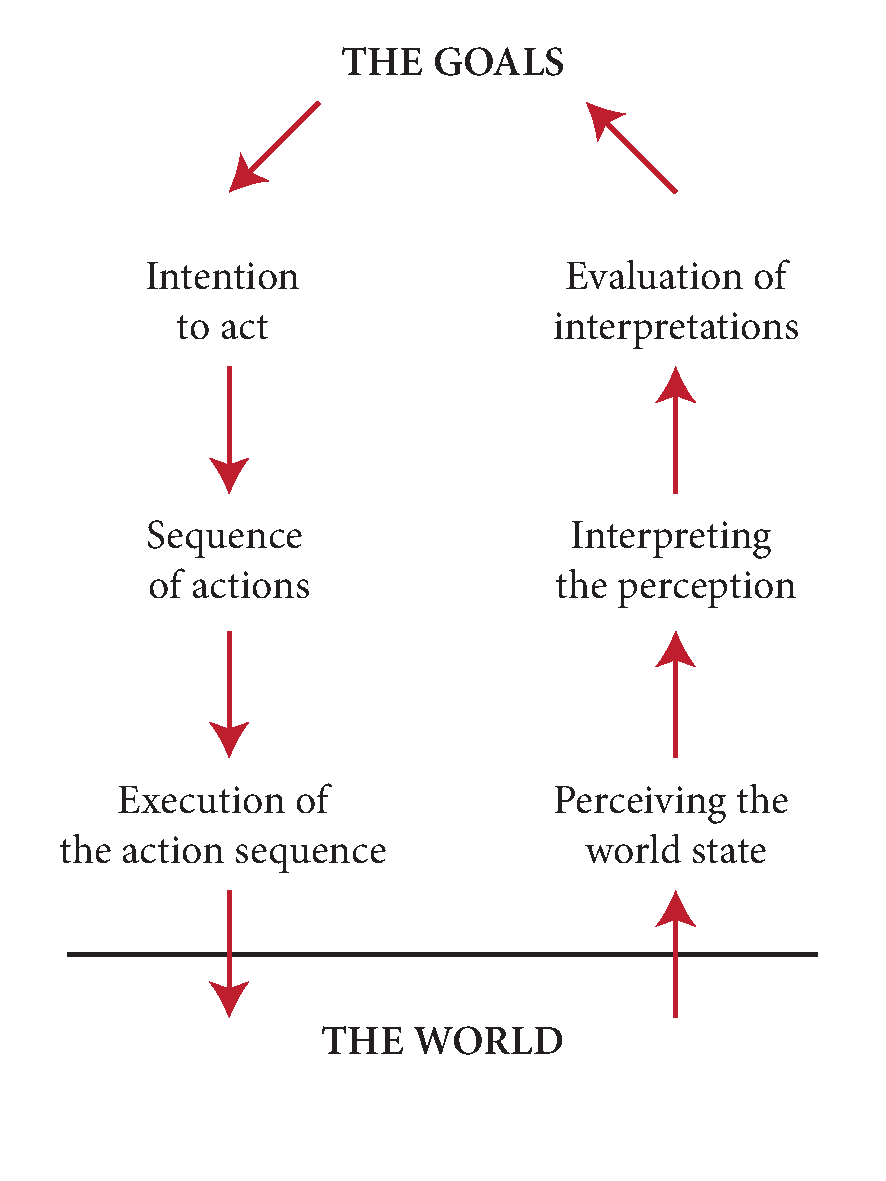
\includegraphics[width=0.5\textwidth]{../graphics/seven-stages.pdf}
    \vspace{-20pt}
    \caption[The Seven Stages of Action]{Stages of Action}
  \end{center}
  \label{fig:seven-stages}
  \vspace{-20pt}
\end{wrapfigure}

Conceptual models used in interaction design can also help us see when and where information overload interferes with a user's experience. 
\cite{Norman1988} advocates a model called \emph{the seven stages of action}, 
that describes how each user goes through several states while using a system
(see Figure \ref{fig:seven-stages}, adapted from \citeauthor{Norman1988}). 
First, the user forms a goal and an intention to act. The user then performs a sequence of actions on the world (the interface)
 meant to align the perceived world and the goals. After performing a set of actions, the new world state is evaluated and perceived. 
At last, the user evaluates the perception and interpretation of the world in accordance with the original goal.

As apparent from this model, information overload can interfere both before and after any action is taken. 
For example, if the application presents too much content, or presents content in a confusing manner, 
it can be difficult for the user to identify which actions that would help achieve the current goal. 
Likewise, after actions are taken, the new world state can suffer the same shortcomings of overwhelming scope or lack of presentations, 
leading to information overload. 
This precludes the user from properly evaluating the resulting application state. 

In short, an application interface can fail both before and after a user tries to interact with it.
Information overload happens throughout the interaction process.


\subsection{Online Overload}

The Web is a common source of information overload, 
and a good example of how and why the problem occurs.
Online information overload is especially pervasive when considering \emph{content aggregating websites}:
Web sites that combine information from multiple other sites and sources. 
Online information retrieval systems (search engines) are in category, as are
online newspapers, feed readers and portal sites.

The wealth and scope of data on the Web are natural culprits of online overload, 
as well as the varying qualities of websites publishing the information. 
However, the problem is also a result of the fundamental observed structure of the Web.
Graph theory presents applicable models that characterize how people navigate between websites, 
and show how content aggregators form important hubs in the network. 
These models give a theoretical foundation for why information overload occurs on the Web.

In the Web graph, nodes correspond to websites and
directed edges between nodes are links from one page to another. The \emph{degree} of a node is defined as its number of edges.
This graph has the properties of a \emph{small-world network} (\citep{Newman2000}, \citep[p2]{Huang2005}), 
a type of random graph, where most nodes are not neighbors, but most nodes are reachable through a small number of edges (See Figure \ref{fig:swn}). 
This is because of important random shortcuts differentiating the graph from a regular lattice. 
The graph is not  random, but neither is it completely regular.
As described by \citet[p37]{Barabasi2003}, the average number of outbound links from a web page is around 7.
From the first page, we can reach 7 other pages. From the second, 49 documents can be reached. 
After 19 links have been traversed, about $10^{16}$ pages can be reached (which is more than the actual number of existing web pages, since loops will form in the graph).
%\footnote{The concept of small-world networks came from the observation that there is often a surprisingly short minimum distance between nodes in an average graph. This is called the small world phenomenon, and is often mentioned alongside the concept of "six degrees of separation", popularized in a play by John Guare. This concept states that no person is on average more than six social links removed from any other person on earth.}

\begin{figure}[t]
  \includegraphics[width=\textwidth]{../graphics/graphs}
  \caption[Examples of Complex Networks]{
    Complex Networks,
    from the left: A \emph{random} network, a \emph{small-world} network and a \emph{scale-free} network 
    (which is a type of  small-world network). Figure adapted from \citep[p2]{Huang2005}.} 
  \label{fig:swn}
\end{figure}


The high degree of the Web graph would suggest that finding an optimal path to your desired page is quite difficult. 
Yet, while it is true that finding the \emph{optimal path} is hard, finding \emph{a good path} is not that big a challenge. 
When people browse the Web, links are not followed blindly --- 
we use numerous heuristics to evaluate each link, often resulting in quite a good path to where we want to go. 
So why is the Web still quite challenging to navigate?

As discovered by \cite{Albert1999}, the Web also exhibits properties of a \emph{Scale-Free Network} (\smallcaps{SFN}). 
They found that in some natural observed networks, there exists a small number of nodes with an extremely high degree. 
This is also true on the Web --- some websites have a huge number of outbound links. 
For comparison, while a random network is similar to a national highway system, with a regular number of links between major cities, scale-free networks are more like an air traffic system, with central hubs connecting many less active airports \citep[p71]{Barabasi2003}.

These highly connected nodes, called \emph{hubs}, are not found in small-world networks or random graphs. As demonstrated by the presence of hubs, the degree distribution of a scale-free network follows a power law, 
$P(k) \sim k^{-\gamma}$, 
where $P(k)$ is the probability of a node having k connections and $\gamma$ is a constant dependent on the type of network, typically in the range $2 < \gamma < 3$. 
Since the Web has directed edges,
we have two power laws:
$P_{in}(k) \sim k^{-\gamma_{in}}$ and 
$P_{out}(k) \sim k^{-\gamma_{out}}$.

\cite{Albert1999} describes a number of studies placing the $\gamma$ values for the Web in the $[2,3]$ range, 
with $\gamma_{out}$ being slightly higher than $\gamma_{in}$. 
Both these probabilities exhibit power tails (or long tails). 
In other words, a few important nodes have a huge number of inbound and outbound links --- the hubs. 
\citet[p86]{Barabasi2003} proposed that hubs emerge in a scale-free networks because of two factors:
(1) Growth: Nodes are added to the network one by one, for example when new websites are added to the Internet.
(2) Preferential attachment: When new nodes are created, they connect to existing nodes. The probability that the new node will connect to an existing node is proportional to the number of links the existing node has. In other words, older, more established and central nodes are preferred neighbors.
This is called the Barab\'{a}si-Albert model \citep{Albert1999}, 
and the probability for a new node connecting to an existing node is given by $\prod k_i$, 
where $k_i$ is the number of links pointing to node $i$, in the following equation: 

\begin{eqsp}
  \prod_{i} k_i  = \frac{k_i}{\sum_{j}^N k_j}.
\end{eqsp} 
%
Search engines, social link aggregators, news portals, et cetera are all hubs of the Internet, emerging from the preferential 
link attachment of newly created nodes, that make navigating the Web less easy as it might appear.
What does seem clear is that these content aggregating hubs are prime candidates for overwhelming their users with information. 
The fundamental observed structure of the Web creates the need for information brokers that link the net together, 
and the need for techniques to display a lot of data --- adapted to each user and each item.
In other words, we need user modeling, that can predict how relevant each item will be for each user.
 


      %\section{User Modeling}
\label{sec:modeling}

The term \emph{user modeling} (\smallcaps{UM}) lacks a strict definition. 
Broadly speaking, when an application is adapted in some way based on what the system knows about its users, we have user modeling. 
From predictive modeling methods in machine learning, 
to how interface design is influenced by personalization, the field covers a lot of ground. 

It is important to differentiate between adapting the interface of an application and the content of an application. 
Many user modeling methods strive to personalize the interface itself, e.g. menus, buttons and control elements 
(e.g. \cite{Jameson2009, Fischer2001}). 
Adapting the content, on the other hand, means changing how and what content is displayed.
For instance, interface adaption might mean changing the order of items in a menu, while content 
adaption might mean changing the order and emphasis of results in a web search interface
(e.g. \cite{Xu2008, Qiu2006, Rhodes2000}).

In this thesis, we are interested in adapting the \emph{content} of an application.
We believe the information overload problem often stems from a mismatch between presented content and desired content. 
Examples of adaptive content include:

\begin{itemize*}
  \item Suggesting interesting items based on previous activity.
  \item Reorganizing or filtering content based on predicted user relevance.
  \item Translating content based on a user's geographical location.
  \item Changing the presentation of content to match personal preferences or abilities.
  \item Personalizing search results based on previous queries and clicks.
\end{itemize*}

The fields of Artificial Intelligence (AI) and Human-Computer Interaction (HCI) share a common goal solving information overload through user modeling. 
However, as described by \cite[p.6]{Lieberman2009}, they have different approaches and their efforts are seldom combined. 
While AI researchers often view contributions from HCI as trivial cosmetics, the HCI camp
tends to view AI as unreliable and unpredictable --- surefire aspects of poor interaction design.

In AI, user modeling refers to algorithms and methods that infer knowledge about a user based on past interaction 
(e.g. \cite{Pazzani2007, Smyth2007, Alshamri2008, Resnick1994}).
By examining previous actions, predictions can be made of how the user will react to future information. This new knowledge is then embedded in a model of the user, which can predict future actions and reactions. 
For instance, an individual user model may predict how interesting an unseen article will be to a user, based on previous feedback on similar articles or the feedback of similar users.

HCI aims to meet user demands for interaction. 
User modeling plays a crucial role in this task. 
Unlike the formal user modeling methods of AI, user models in HCI are often cognitive approximations, manually developed by researchers to describe different types of users 
(e.g. \cite{Fischer2001, Jameson2009, Cato2001}).
These models are then utilized by interaction designers to properly design the computer interface based on a models predictions of its user's preferences.
\cite{Totterdell1990} describes user modeling in interaction design as a collection of deferred parameters: 

\begin{blockquote}
  ``The designer defers some of the design parameters such that they can be selected or 
  fixed by features of the environment at the time of interaction [...] 
  Conventional systems are special cases of adaptive systems in which the parameters have been pre-set.'' 
\end{blockquote}

This thesis is concerned with the AI approach to user modeling, and in particular, the use of \emph{recommender systems} (RSs).

\subsection{Interface Autonomy}

\begin{figure}[t]
  \includegraphics[width=\textwidth]{../graphics/autonomy.pdf}
  \caption[Levels of Interface Autonomy]{
    Levels of Interface Autonomy:
    Interfaces range from those only customizable by the user, 
    to intelligent systems takes the initiative on their own accord.
  }
  \label{fig:autonomy}
\end{figure}

Using AI to adapt an interface raises important questions with regard to usability, privacy and usefulness.
These questions are rooted in the autonomy expressed by each interface.
An autonomous interface is one that takes initiatives on its own, regardless of whether the user has asked for it \cite[p.2]{Lieberman}. 
Naturally, any application that automatically personalizes its content will be autonomous to some degree.

Adaptive interfaces can be classified into increasing order of autonomy (see Figure \ref{fig:autonomy}). 
At the order of least autonomous systems, we have \emph{customizable interfaces}. 
These are interfaces that the user may customize themselves, but that do not take the initiative or change anything without explicit user action. 
For example, an interface might have a settings panel where users can change the order of items in a menu.

At the next level of autonomy, we have \emph{adaptive interfaces} that suggest to the user possible changes or actions that might be beneficial. For example, an email application could suggest which folder an email should be moved to.
At the most autonomous level, \emph{intelligent interfaces} implicitly and automatically customize the interface or content based on passive observation of the user. 
This could for instance entail automatic filing of emails based on content classification and data mining of previous user actions with similar messages.

An application that personalizes content automatically will fall somewhere in the two last categories and present either an adaptive or intelligent interface, 
depending on the extent and transparency of its autonomy.

In this thesis, we are only interested in fully autonomous, intelligent interfaces.
We will create a system that implicitly, and without any effort from each user,
can adapt the content of an application based on previous behavior.
Other examples of such implicit user modeling include \cite{Qiu2006}, \cite{Shen2005} and \cite{Carmel2009}.

As our goal is to adaptively combine different RSs based on each user and item,
we shall now describe what makes a recommender system, and introduce some of the many algorithms they employ.

      %\section{Recommender Systems}

The name might seem constraining, but recommender systems are incredibly powerful methods in user modeling.
Whenever we wish to predict the relevance of an item to a user, recommender systems are the tools to use.
Such systems are commonly used on the web to provide a host of predictive functionality, including:

\begin{itemize*}
  \item Recommending products like books or movies based on past purchases.
  \item Suggesting new social connections based on an existing social graph.
  \item Recommending items based the activity of similar or like-minded users.
  \item Ordering news articles by predicted individual relevance.
\end{itemize*}

Common to these examples are a set of users, a set of items, and a sparse set of explicit ratings or preferences.
A recommender system is best described as a graph, even though the underlying algorithms might not use this as the representation.
\cite{Mirza2003} explains how any RS can be expressed as a graph traversal algorithm.
Items and users are nodes, while ratings, social connections et cetera are edges between the nodes.
An RS performs predictive reasoning on this graph by estimating the strenghts of hypothetical connections between nodes that are not explicitly connected.

For example, if a user has rated some of the movies in a movie recommendation system, 
we use these ratings to predict how well the user will like unseen movies,
based on a movies ratings from users similar to the one in question.
In social networks, recommender systems can be used to infer new social relations 
based on existing connections. The principle is the same: By evaluating current explicit
connections, and the connections of similar users, new connections can be predicted.
Recommender systems are then powerful methods for user modeling, personalization and fighting information overload,
because of their ability to infer how relevant and item (or another user) will be to the current user.

Formally, a recommender system is a quintuple, $\mathrm{RS} = (I, U, R, F, M)$,
where $I$ is the set of items (e.g. products, articles or movies) and $U$ is the set of users.
$R$ is the set of known ratings, i.e. explicit preferences given by users for certain items.
$F$ is a framework for representing the items, users and ratings, and 
$M$ is the actual modeling method used to infer unknown ratings 
for predicting a user's preference for an unrated item. 

In \cite{Adomavicius2005}, $M$ is seen as a utility function
$f: U \times I \rightarrow S$. Here, $f$ is a function that maps the set
of users and items into a fully ordered set of items $S$, ranked by their
utility (i.e. rating) to each user. In other words, $S$ is the complete version of $R$,
where each user has either an explicit or predicted preference for each item in $I$.
In this notation, to predict the best unrated item for each user, we simply find the item with the highest expected utility:

\begin{eqnarray*}
  \forall u \in U,\text{ } i'_u = \arg\max_{i \in I} f(u,i)
\end{eqnarray*}

The utility function $u$ depends on the modeling method being used, the active user and the item in question. 
The \emph{reason} for using a recommender system is that the utility $u$ is not defined for the entire $U \times I$ space, 
i.e. the system does not explicitly know the utility of each item for each user. 
The point of a recommender system is then to extrapolate $u$ to cover the entire user-item space. 
In other words, to be able to rank items according to user preferences, 
the system must be able to predict each user's reaction to items they have not yet explicitly rated themselves. 
This is where predictive user models come in handy.

Another popular way of describing, and implementing an RS is using a simple matrix. 
Here, one dimension represents users, the other dimension represents items,
and each cell corresponds to an explicit rating. This matrix then becomes the framework $F$ in our 
RS quintuple:

\begin{eqnarray*}
 R_{m,n} =
 \begin{pmatrix}
  r_{1,1} & r_{1,2} & \cdots & r_{1,n} \\
  r_{2,1} & r_{2,2} & \cdots & r_{2,n} \\
  \vdots  & \vdots  & \ddots & \vdots  \\
  r_{m,1} & r_{m,2} & \cdots & r_{m,n}
 \end{pmatrix}
\end{eqnarray*}

Critically, these matrices are usually extremely sparse (i.e. most of the cells are empty). 
Consider that while there may be a large number of users and items, each individual user
only rates or connects to a few number of items. 
For example, in the seminal Netflix Challenge movie recommender dataset, almost 99\% of the potential
user/item pairs have no rating \citep[p1]{Bell2007d}. In other words, the recommender system must be able
to produce results from a matrix where only 1\% of the cells have meaningful values.

Naturally, this is the defining characteristic of 
many recommender systems: the ability to extract meaningful patterns from sparse data, 
through dimensionality reduction, neighborhood estimation and similar methods.

Recommender systems face many challenges other than the sparsity problem.
A directly related problem is the need for large datasets. Since the data is often sparse,
the systems will most often perform well if used on large numbers of items and users.
As in many machine learning methods, concept drift, where the characteristics of a user or item
changes over time, is also eternally present.
Finally, the performance of RSs is often closely tied to their computational complexity. 
Real world usage of the most precise methods is often hindered by the computational power
needed to actually put them into production.




\subsection{Estimation of Ratings}

The most interesting and important part of any RS is how it predicts unknown ratings.
(Note that altough we use "ratings", "utility", "preference", "relevance" and "connection strength" depending on the context, they all basically mean the same.)
Because of this, each method is best categorized based on a few dimensions of its predictive capabilities (see Table \ref{table:taxonomy}).
In our taxonomy, these dimensions are: Predictions, method, granularity, temporality and agents.

\begin{table}[b]
  \begin{tabular*}{\textwidth}{ p{3cm} l @{\extracolsep{\fill}} }
    \toprule
    \emph{Variable} & \emph{Values} \\
    \midrule
    Predictions & Content-based | Collaborative | Hybrid\\
    Method & Heuristic | Model-based\\
    Granularity & Canonical | Typical | Individual\\
    Temporality & Short-term | Long-term\\
    Agents & Implicit | Explicit\\
    \bottomrule
  \end{tabular*}
  \caption[Recommender Systems Taxonomy]{A taxonomy of recommender systems. From \cite{Bjorkoy2010d}.}
  \label{table:taxonomy}
\end{table}

The \emph{predictions} variable represents what data the RS uses to perform predictions. 
Content-based methods use only the items, inter-item relations, and 
an individual user's past history as predictive of future actions \citep{Pazzani2007}.
By only considering the individual user in adapting an application, highly personal models can be created. 
However, such methods often require a lot of interaction before reliable models can be created \citep{Adomavicius2005}.
The problem of having to do complex inference from little data, as is often is in content-based predictions, is often called the \emph{sparsity problem} or the \emph{cold start} problem. This is closely related to the problem of \emph{overfitting} data, where the algorithms creates models that match the training data, but not the actual underlying relationships. A lot of research looks at ways to overcome sparse data, i.e. achieving "warmer" cold start. 
When using content-based predictions, the utility function $f(u,i)$ of user $u$ and item $i$ is extrapolated from $f(u,i_u)$, 
where $i$ is an item similar to $i_u$ and $f(u,i_u)$ is known.

Collaborative or social recommendations build predictive models for users based on the actions of similar users 
\citep{Schafer2007}.
The observation is that similar users should have similar usage and action patterns. 
By using data from more than one user, expansive models may be built. 
These methods are especially useful when considering new users of a service. 
A central problem with collaborative methods is that the resulting model is not as individually tailored as one created through content-based learning. 
Collaborative models must be careful not to represent the \emph{average} user, but a single individual.
When using collaborative learning, 
the utility $f(u,i)$ of item $i$ for user $u$ is extrapolated from $f(u_j,i)$ where $u_j$ is a user similar to $u$. 

Because of \emph{the new user problem} of content-based learning and the \emph{average user problem} of collaborative learning, 
many systems use a hybrid approach \citep{Burke2007}.
By combining content-based and collaborative learning, 
systems that properly handle predictions for new users and avoid too much generalization in the models can be achieved. 

The \emph{method} variable, is another way to classify recommenders. Orthogonal to what data the method uses, this variable
concerns \emph{how} the data is used to produce recommendations.
First we have the \emph{model-based} approach, where the recommender system builds predictive models based on the known data. 
Unseen items can then be fed into this model to compute its estimated utility score. 
For example, creating a Bayesian networks from past interaction is a model-based approach.
The other category is the \emph{heuristic} or \emph{memory-based} approach. 
These methods use the raw data of items, users and ratings to directly estimate unknown utility values. 
For example, recommending items similar to the ones already rated by computing the cosine similarity of their feature vectors is a heuristic approach.


The \emph{granularity} variable tells whether this approach creates models for the canonical user, stereotypical users or individual users. 
\cite{Rich1979} presented one of the first user modeling systems based on stereotypes, used to predict which books in a library each user would most enjoy.
Here, a dialogue between the system and the user was performed to place the user into a set of sterotypes. 
Each stereotype has a set of \emph{facets} which is then used to match books and users.

\emph{Temporality} refers to how volatile the gathered knowledge will be.
While most RSs produce long term, relatively stable knowledge based on lasting user preference and taste, 
some systems use fluctuating parameters such as the time of day, exact location and the current context to produce recommendations.
For example, \cite{Horvitz} used clues from a user's calendar, camera and other sensors to determine the attentional state
of the user before delivering personalized and contextual notifications.

The \emph{agents} variable signifies whether the knowledge gathering and presentation is implicit and opaque, 
or explicit and requires dedicated user interaction. Explicit feedback through ratings is 
common in movie, product or music rating services (e.g. \cite{Bell2007, Basu1998, Hotho}). However, for other services such as personalized search,
implicit mining of query logs and user interaction is often used to build user models (e.g. \cite{Shen2005, Agichtein2006, Speretta2000, Teevan2005})


\subsection{Approaches}

Because our solution will combine different recommender systems, we need a short introduction to some of the approaches we will combine.

TODO

      \section{Personalized Search}

Information retrieval (+ information overload)

An Information Retrieval Model is a quadruple \citep[p23]{Baeza-Yates1999}:

\begin{eqnarray}
  \mathrm{IR} = (Documents, Queries, Framework, ranking(q_i, d_i))
\end{eqnarray}

Common metrics

Personalized metrics

Relation to recommender systems




      
\section{Aggregate Modeling}

\begin{eqnarray}
  \mathrm{AM} = (Items, Users, Framework, Methods, Aggregation)
\end{eqnarray}

Getting past 80\%

Power of data

Current methods (non-personal)

Use cases (netflix, ...)

For personalized search (speculation)

Hypotheses

Explain next chapter



 
    %\chapter{Methods}
    %  \section{Modeling}



\section{Composition}      

\subsection{Reverse Map Stage}

\subsection{Reduce Stage}



\section{Application}



\section{Implementation}      

\subsection{Personalized Search}

\subsection{Information Retrieval}

\subsection{Modeling Algorithms}

\subsection{Composition}



\section{Evaluation}   

\subsection{Datasets}

\subsection{Metrics}

\subsection{Experiments}




    %\chapter{Results}
    %  \section{Experiments}      
\section{Results}      
\section{Discussion}      




    %\chapter{Conclusion}
    %  \label{chap:discussion}

This chapter will discuss the implications of our results.
While our hypotheses may be answered,
it is important to clarify what we have actually found out,
and what limits there is to this knowledge.
We will also summarise the contributions of this paper,
and suggest possible future work.


\section{Implications}      

Our central position is that modern aggregate recommender systems 
are constrained by misplaced subjectivity.
Each system selects some measures to model its users, while this selection should be left to each user.
This problem extends to the items recommended by each system: 
Different modeling methods will suit each item differently.

Stacked recommenders can help solve this problem.
In a collection of possible recommender algorithms, each is adaptively used based 
on how well it performs for the item and user in question.
We think the experiments in the previous chapter shows the promise of this technique.
However, there are lots of use cases not yet considered.

It should be clear that stacked recommenders would work best in situations where
we have a wide range of diverse algorithms that can infer the relevance of an item to a user.
For users, social connections is a good example: whether or not social connections should influence
recommendations or personalized search results is a contentious topic.
Naturally, a system where each user's personal opinion determines if these connections are used is desireable.

This implication extens to the items that should be recommended:
As evident by the field of information retrieval,
there exists many ways of considering the relevance of an item. 
Each of these algorithms can be based on a number of attributes:
temporality, geography, sentiment analysis, topic or key words.
It is not a huge leap to consider that each of these algorithms may have
varying levels of accuracy for each individual item.
Stacked recommenders can help solve this problem by adaptively 
combining the recommenders based on individual item performance.

With stacked recommenders, both the methods layer and the adaptive layer consists of standard recommender algorithms.
Because we use ratings matrices for the taste models and error matrices for the weight estimations,
we can use the same algorithms for both tasks.
Using known algorithms for this new task is beneficial:
they are known to work, enjoy multiple implementations
and are already understood and battle-tested in many different systems.

However, as this approach is more complicated than standard recommenders,
it is worth questioning if its gains are worth the extra complexity.
This depends on the basic recommenders that are to be combined.
If the system is made up by many different recommenders,
that each user might place varying importance on,
and that may have varying success with each item,
stacked recommenders may provide implressive gains in accuracy.
On the other hand, if the recommenders are simple in nature,
and look at similar patterns in the data,
generalized aggregation methods might be more applicable.




\section{Contributions} 

We have made two main contributions with this paper:
(1) described the latent subjectitivty problem and
(2) developed the technique of stacked recommenders.

(1) The latent subjectivity problem is one we think hinders
standard recommender systems reaching their full potential.
As far as we know, this problem has not been described
in the context of recommender systems.
The main choice for any such system is how to predict unknown ratings.
To do this, a pattern in the available ratings data must be leveraged.
These patterns are plentiful, and which works best is dependent on
each user and item in the system.
Modern aggregation recommenders utilize many patterns, but on a generalized
level, where each user and item is treated the same.
This underlying subjectivity leads to a mismatch between the notions
of whoever developed the systems, and the users and items of the service.

The latent subjectivity problem extens to any ensemble learning systems
(as those described in \cite{Polikar2006}) that blends multiple 
algorithms to leverage patterns.
Whenever we have multiple algorithms that work on a set of items
(and possibly users), there is a question of how accurate each
approach will be for each item.
Averaged or generalized weighted approaches will always
chose the combination that performs best \emph{on average},
with little concern to the uniqueness of items (and users).
In other words, this is a comprehensive problem
that may be discovered amongst many machine learning techniques.

(2) Stacked recommenders is our attempt to solve the latent subjectivity problem.
As far as we know, this type of adaptive prediction aggregation has not been done before.
Chapter \ref{chap:results} showed that an aggregation that combines predictions based
on estimated accuracy can outperform both standard recommenders and simple aggregation approaches.
Our technique is strengthened by the fact that standard recommender algorithms
are used for the accuracy estimations.
This is the core insight of this paper: 
by creating error models for each recommender, we can use this to predict
its accuracy for each user/item combination.
These predictions can then be used to weigh each combined algorithm accordingly.

As far as the latent subjectivity problem extends to any ensemble learning system,
the adaptive aggregation part of stacked recommenders can be used to 
create better combinations of many types of predictors.
Whenever we have a set of algorithms producing a set of predicted values
based on items, a set of aggregating recommenders can model the probable
errors of these approaches, based on each individual item.
This leads to adaptive ensembles that should outperform generalized approaches.
Because of this, the technique build in this paper should be 
applicable in situations other than recommender systems.

While the experiments of Chapter \ref{chap:results} show the general viability of stacked reocmmenders,
we belive there are greater opportunities in systems where there  are even more diverging
patterns to be leveraged. The prime examples of this are systems that may or may 
not use social connections between users, and systems which predict the 
relevance of widely varying items.


\section{Future Work}      

We have only shown the basic viability of stacked recommenders,
and how they can outperform traditional approaches on traditional datasets.
This section outlines a few interesting research topics
which should shed more light on the subject.

\subsection{Different adaptive recommenders}

We chose to use SVD-based recommenders for the adaptive part of our stacked approach.
The main reason for this is that we are looking for global traits of the data
when performing accuracy estimations. In other words, we wish to identify
clusters of users and items for which each algorithm may or may not be suited.

However, as the stacked recommenders can utilize any standard recommender system
to model the errors of another recommender, it would be interesting to perform
a more in-depth study of how different choices for the adaptive layer
influence the final system.
There are many more recommenders that also look at global patterns
that might be well suited for this task.


\subsection{Different domains}

We chose to use the MovieLens dataset and the RMSE evaluation measure for testing our approach.
The primary reason was to be able to direcly evaluate our results towards those of other research papers.
As this dataset and this error measure is widely used to evaluate recommender systems,
it is natural for a first look at a new approach to use the same notions of accuracy.

However, as mentioned above, the main strength of stacked recommenders may be
in situations with much more diverse data sources. Social networks or systems
with widely varying sets of items would provide an interesting use case for stacked recommenders.
The main premise of our approach is that each user and item have differing preferences
for each algorithm. Naturally, the more diverse the data and algorithms get,
the more dire the need for adaptive aggregation becomes.
Because of this, using stacked recommeners in other domains with more variation 
in the data and combined algorithms would be an interesting topic.


\subsection{Different fields}

We have only considered the notion of latent subjectivity within the field of recommender systems.
However, as briefly mentioned above, the technique should be applicable to many more situations.
Whenever there is a set of prediction algorithms that use different data to produce results,
an adaptive aggregation should be able to combine these in a more nuanced way.

Ensemble learning is a big topic, used in many situations.
By stacking recommenders on top of each method in an ensemble, 
we get a system capable of predicting the accuracy of each method.
Naturally, it would be interesting to see how this approach would fare
in other fields such as document classification, document clustering,
curve fitting \cite[p7]{Polikar2006}, and any other field of ensemble learning.


\section{Conclusion}      




  \backmatter
    {
  %\footnotesize

  \bibliographystyle{apalike}      
  %\bibliographystyle{plain}      

  \bibliography{library}
}

    %\begin{appendices}
    %  \addtocontents{toc}{\protect\setcounter{tocdepth}{0}}

\chapter{Implementation Details}

lorem

\section{Hadoop}
\section{Mahout}
\section{JRuby}

\chapter{Expanded Results}

lorem


\chapter{Resources}

    %\end{appendices}
    
\end{document}

